\documentclass[12pt,a4paper]{article}
\usepackage{amsmath,amsfonts,amssymb}
\usepackage{graphicx}
\usepackage{enumitem}
\usepackage[dvipsnames]{xcolor}
\usepackage{pgfplots}
\usepackage{hyperref}
\usepackage{soul}
\usepackage{framed}
\usepackage{booktabs} 
\usepackage{tabularx}
\usepackage{array}

\definecolor{lessonbgcolor}{rgb}{0.9,0.9,1}
\definecolor{examplecolor}{rgb}{0.8,1,0.8}
\definecolor{noteboxcolor}{rgb}{1,0.8,0.8}
\newenvironment{lesson}[1]
  {\begin{framed}\colorbox{lessonbgcolor}{
  \parbox{\dimexpr\linewidth-2\fboxsep}{
  \textbf{#1}}}\end{framed}}
  
\newenvironment{example}
  {\begin{framed}\colorbox{examplecolor}{
  \parbox{\dimexpr\linewidth-2\fboxsep}{
  \textbf{Example:}}}}
  {\end{framed}}
\newenvironment{note}
  {\begin{framed}\colorbox{noteboxcolor}{
  \parbox{\dimexpr\linewidth-2\fboxsep}{
  \textbf{Note:}}}}
  {\end{framed}}
\begin{document}
\section*{Unit 3: Quadratic Functions}
Quadratic functions are a class of polynomial functions of the form $f(x) = ax^2 + bx + c$, where $a$, $b$, and $c$ are constants, and $a$ is not equal to zero. They play a crucial role in algebra, calculus, physics, engineering, and various other fields. 
\section{The Standard Form of Quadratic Functions}

A quadratic function is typically expressed in standard form as:

\begin{equation}
f(x) = ax^2 + bx + c
\end{equation}

Here is a brief explanation of the parameters:

\begin{itemize}
    \item $a$: The coefficient of the quadratic term. It determines the direction in which the parabola opens (upwards if $a > 0$, and downwards if $a < 0$).
    \item $b$: The coefficient of the linear term. It shifts the vertex of the parabola horizontally.
    \item $c$: The constant term. It shifts the vertex of the parabola vertically.
\end{itemize}

\section{Vertex Form of a Quadratic Function}

The vertex form of a quadratic function is particularly useful for identifying the vertex and other properties. It is expressed as:

\begin{equation}
f(x) = a(x - h)^2 + k
\end{equation}

In this form, the vertex of the parabola is represented by the point $(h, k)$.
\newpage
\section{Vertex and Axis of Symmetry}

The vertex of a quadratic function in standard form ($f(x) = ax^2 + bx + c$) can be determined using the following formulas:

\begin{align}
x_{\text{vertex}} &= \frac{-b}{2a} \\
y_{\text{vertex}} &= f(x_{\text{vertex}})
\end{align}

In vertex form ($f(x) = a(x - h)^2 + k$), the vertex is already given as $(h, k)$.

The axis of symmetry is a vertical line that passes through the vertex. It is given by the equation:

\begin{equation}
x = \frac{-b}{2a}
\end{equation}

\section{Discriminant and Solutions}

Quadratic functions may have real or complex solutions. The discriminant ($\Delta$) can be used to determine the nature of the solutions:

\begin{equation}
\Delta = b^2 - 4ac
\end{equation}

The solutions are classified as follows:

\begin{itemize}
    \item If $\Delta > 0$, the function has two distinct real solutions.
    \item If $\Delta = 0$, the function has one real solution (a repeated root).
    \item If $\Delta < 0$, the function has two complex solutions.
\end{itemize}
\section{Graph of a Quadratic Function}

A graphical representation of a quadratic function helps us visualize its behavior. Let's consider an example:

\begin{equation}
f(x) = 2x^2 - 3x + 1
\end{equation}

\subsection{Vertex Calculation}

Using the formulas, we can find the vertex:

\begin{align*}
x_{\text{vertex}} &= \frac{-(-3)}{2(2)} = \frac{3}{4} \\
y_{\text{vertex}} &= f\left(\frac{3}{4}\right) = 2\left(\frac{3}{4}\right)^2 - 3\left(\frac{3}{4}\right) + 1 = \frac{7}{8}
\end{align*}

So, the vertex of the quadratic function is $\left(\frac{3}{4}, \frac{7}{8}\right)$.
\subsection{Graph}

You can visualize the graph of the quadratic function:

\begin{center}
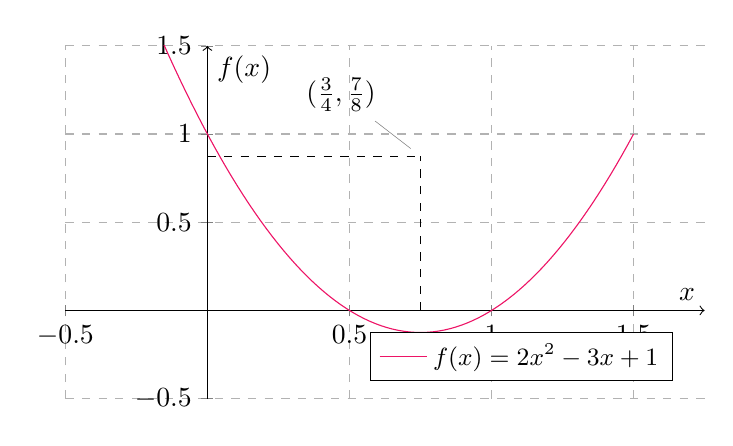
\begin{tikzpicture}
    \begin{axis}[
        xlabel=$x$,
        ylabel=$f(x)$,
        xmin=-0.5, xmax=1.75,
        ymin=-0.5, ymax=1.5,
        axis lines=middle,
        axis line style={->},
        legend style={at={(0.95,0.05)},anchor=south east},
        grid=both,
        major grid style={dashed,gray!60},
        width=0.8\textwidth,
        height=0.5\textwidth,
        legend style={font=\small},
        legend cell align={left},
    ]
    \addplot[WildStrawberry,domain=-0.5:1.5, samples=100] {2*x^2 - 3*x + 1};
    \legend{$f(x) = 2x^2 - 3x + 1$}
    
    \node[pin=135:{$(\frac{3}{4}, \frac{7}{8})$}] at (axis cs:0.75,0.875) {};
    \draw[dashed] (axis cs:0.75,0) -- (axis cs:0.75,0.875);
    \draw[dashed] (axis cs:0,0.875) -- (axis cs:0.75,0.875);
    
    \end{axis}
\end{tikzpicture}
\end{center}

\subsection*{\hl{Remember!}}

\begin{minipage}{\textwidth}
\textbf{Parabolas (Standard Form)}

\begin{tabularx}{\textwidth}{|X|X|}
\hline
\textbf{Equation} & $y = ax^2 + bx + c$ \\
\hline
\textbf{Vertex} & $(-\frac{b}{2a}, -\frac{b^2-4ac}{4a})$ \\
\hline
\textbf{Opening Direction} & Down if $a > 0$ \\
\hline
\textbf{Y-intercept} & $(0, c)$ \\
\hline
\end{tabularx}

\textbf{Parabolas (Vertex Form)}

\begin{tabularx}{\textwidth}{|X|X|}
\hline
\textbf{Equation} & $y = a(x - h)^2 + k$ \\
\hline
\textbf{Vertex} & $(h, k)$ \\
\hline
\textbf{Opening Direction} & Up if $a > 0$, Down if $a < 0$ \\
\hline
\end{tabularx}
\end{minipage}

\newpage
\section{Applications of Quadratic Functions}

Quadratic functions are not merely theoretical; they have numerous practical applications in various fields. Some common applications include:

\begin{enumerate}
    \item \textbf{Physics}: Quadratic functions describe the motion of objects under the influence of gravity. The equation $h(t) = -16t^2 + v_0t + h_0$ models the height ($h$) of an object at time ($t$) when it is thrown vertically with an initial velocity ($v_0$) from an initial height ($h_0$).

    \item \textbf{Engineering}: In structural engineering, quadratic equations model the deformation of materials under load, helping engineers design stable structures.

    \item \textbf{Economics}: Quadratic functions are used to model cost, revenue, and profit functions in business and economics. These functions assist in optimizing production and pricing strategies.

    \item \textbf{Computer Graphics}: In computer graphics, quadratic functions are used to create smooth curves and surfaces. For instance, Bézier curves are defined using quadratic equations.

    \item \textbf{Biology}: Quadratic functions can model population growth or decline of species. The logistic growth model is an example of such an application.

    \item \textbf{Statistics}: In regression analysis, quadratic functions are used to model complex relationships between variables.

    \item \textbf{Astronomy}: Quadratic equations can describe the orbits of celestial bodies and the motion of planets.

\end{enumerate}

\subsection*{Note}

Quadratic functions are versatile and play a fundamental role in mathematics and various scientific disciplines. Understanding their properties, equations, and applications is crucial to problem solving and modeling real-world phenomena. Whether in physics, engineering, economics, or any other field, the knowledge of quadratic functions is a valuable asset in tackling complex problems.
\end{document}
